%%%%%%%%%%%%%%%%%%%%%%%%%%%%%%%%%%%%%%%%%%%%%%%%%
% Introduction
%%%%%%%%%%%%%%%%%%%%%%%%%%%%%%%%%%%%%%%%%%%%%%%%%
\subsection{Introduction}
\label{zynq:introduction}
\nocite{Zynq7000:ProductBrief,Zynq7000:UserGuide}
In this Thesis, the \gls{FPGA} that was used was a Xilinx\textregistered
\verb+Z7020CLG484-1+ from the Zynq-7000 product series. This device has an
Arm\textregistered dual-core Cortex\texttrademark-A9 processor, as well as
Xilinx 28nm programmable logic. An image of a Xilinx\textregistered Zynq-7000
series device is shown in \autoref{fig:zynq:z702}.

\begin{figure}
    \centering
    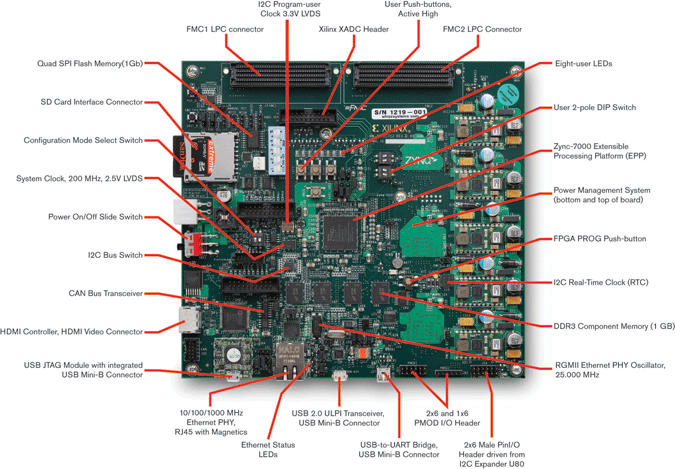
\includegraphics[width=0.5\textwidth]{xilinx/zc702-base-board}
    \caption{A Xilinx ZC7020 \gls{FPGA}.}
    \label{fig:zynq:zc702}
\end{figure}

%%%%%%%%%%%%%%%%%%%%%%%%%%%%%%%%%%%%%%%%%%%%%%%%%
% Board Features
%%%%%%%%%%%%%%%%%%%%%%%%%%%%%%%%%%%%%%%%%%%%%%%%%
\subsection{Board Features}
\label{zynq:features}
\nocite{Zynq7000:UserGuide}
\begin{itemize}
    \item Zynq-7000 XC7Z020-1CLG484C \gls{EPP}
    \item 1 GB \gls{DDR}3 component memory (four 256 Mb x 8 devices)
    \item 128 Mb Quad \gls{SPI} flash memory
    \item \gls{USB} 2.0 ULPI (UTMI+ low pin interface) transceiver
    \item \gls{SD} connector
    \item \gls{USB} \gls{JTAG} interface via Digilent module
    \item Clock sources:
    \begin{itemize}
        \item Fixed 200 MHz \gls{LVDS} oscillator (differential)
        \item \gls{I2C} programmable \gls{LVDS} oscillator (differential)
        \item Fixed 33.33 MHz \gls{LVCMOS} oscillator (single-ended)
    \end{itemize}
    \item Ethernet \gls{PHY} \gls{RGMII} interface with RJ-45 connector
    \item \gls{USB}-to-\gls{UART} bridge
    \item \gls{HDMI} codec
    \item \gls{I2C} bus
    
    \item \gls{I2C} bus multiplexed to:
    \begin{itemize}
        \item Si570 user clock
        \item ADV7511 \gls{HDMI} codec
        \item M24C08 \gls{EEPROM} (1 kB)
        \item 1-To-16 TCA6416APWR port expander
        \item RTC-8564JE real time clock
        \item FMC1 LPC connector
        \item FMC2 LPC connector
        \item \gls{PMBUS} data/clock
    \end{itemize}
    \item Status \glspl{LED}:
    \begin{itemize}
        \item Ethernet status
        \item Power good
        \item FPGA INIT
        \item FPGA DONE
    \end{itemize}
    \item User \gls{IO}:
    \begin{itemize}
        \item Eight user \glspl{LED}
        \item Two \gls{PL} user pushbuttons
        \item \gls{PL} user \gls{DIP} switch (2-pole)
        \item Two \gls{PS} pushbuttons shared with \gls{PS} 2-pole \gls{DIP}
            switch
        \item Two \gls{PS} user \glspl{LED}
        \item Dual row Pmod \gls{GPIO} header
        \item Single row Pmod \gls{GPIO} header
    \end{itemize}
    \item \gls{EPP} \gls{PS} Reset Pushbuttons:
    \begin{itemize}
        \item SRST_B \gls{PS} reset button
        \item POR_B \gls{PS} reset button
    \end{itemize}
    \item Two VITA 57.1 FMC LPC connectors
    \item Power on/off slide switch
    \item Power management with \gls{PMBUS} voltage and current monitoring via
        TI power controllers
    \item Dual 12-bit 1 MSPS XADC analog-to-digital front end
    
    \item Configuration options:
    \begin{itemize}
        \item Quad \gls{SPI} flash memory
        \item \gls{USB} \gls{JTAG} configuration port (Digilent module)
        \item Platform cable header \gls{JTAG} configuration port
        \item 20-pin \gls{PL} \gls{PJTAG} header
        \item 20-pin \gls{PL} \gls{JTAG} header
    \end{itemize}
\end{itemize}

\begin{figure}
    \centering
    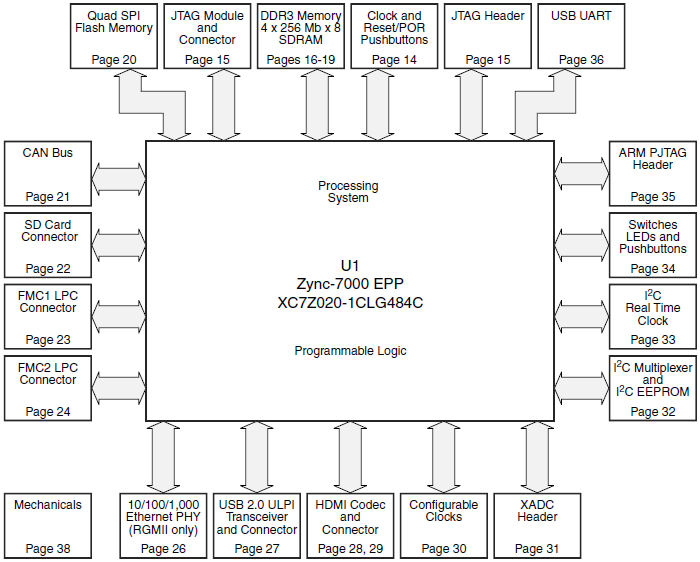
\includegraphics[width=0.5\textwidth]{xilinx/block-diagram}
    \caption{A block diagram for the Xilinx Z7020 series \glspl{FPGA}.}
    \label{fig:zynq:blockDiagram}
\end{figure}
